\subsection{Is the one-pass probability calibrated?}
\label{sec:calibration}
\begin{table}[t]
\centering\small
\caption{Calibration of JEV-9B System~1's top probability by task family: mean confidence, accuracy, their gap (overconfidence, points) and expected calibration error (15 bins).}
\label{tab:calibration}
\begin{tabular}{@{}lrrrrr@{}}
\toprule
Family & $n$ & Mean conf. & Accuracy & Over-conf. & ECE \\
\midrule
anli & 1200 & 73.0 & 64.2 & 8.8 & 0.105 \\
controlled & 488 & 66.9 & 56.1 & 10.7 & 0.116 \\
folio & 204 & 76.4 & 69.6 & 6.8 & 0.098 \\
halueval & 1000 & 89.0 & 82.7 & 6.3 & 0.067 \\
judgebench & 349 & 75.5 & 68.2 & 7.3 & 0.085 \\
rewardbench & 2984 & 88.5 & 87.0 & 1.5 & 0.026 \\
\bottomrule
\end{tabular}
\end{table}

\begin{figure}[t]
\centering
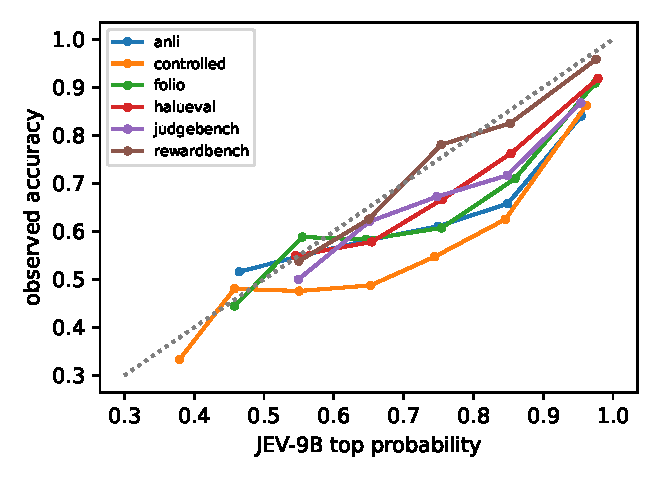
\includegraphics[width=0.55\linewidth]{figures/calibration.pdf}
\caption{Reliability of JEV-9B System~1's top probability by task family (bins with at least 15 items).}
\label{fig:calibration}
\end{figure}
A decision model's selling point is its probability, so we test it out of distribution (Table~\ref{tab:calibration}, Figure~\ref{fig:calibration}).
On RewardBench the top probability is well calibrated (mean confidence 88.5\% against 87.0\% accuracy; ECE 0.026).
On the reasoning panels it is systematically overconfident by 6.8 (FOLIO) to 10.7 (controlled) points, with ECE around 0.10---two orders of magnitude above the 0.0007 the model card reports on its in-distribution test set.
Confidence remains informative for ranking (it is what makes the JEV-H gate work), but a deployment should not read a 0.8 from JEV-9B on a reasoning task as an 80\% chance of being right without recalibrating on its own data.
